\documentclass[10pt,oneside]{article}
\usepackage[T1]{fontenc}
\usepackage[utf8]{inputenc}
% \usepackage{lmodern}
%\usepackage[adobe-utopia,uppercase=upright,greeklowercase=upright]{mathdesign}
\usepackage[adobe-utopia]{mathdesign}
%\usepackage{minionpro}
% \usepackage{pifont}
% \usepackage{amssymb}
\usepackage{amsmath}
\usepackage[francais]{babel}
% \usepackage[francais]{varioref}
\usepackage[dvips]{graphicx}

\usepackage{framed}
\usepackage[normalem]{ulem}
\usepackage{fancyhdr}
\usepackage{titlesec}
\usepackage{vmargin}
\usepackage{longtable}

\usepackage{ifthen}


%\usepackage{epsfig}
\usepackage{subfig}

\usepackage{multirow}
\usepackage{multicol} % Portions de texte en colonnes
\usepackage{flafter}%floatants après la référence



\usepackage{color}
\usepackage{colortbl}


\definecolor{gris25}{gray}{0.75}
\definecolor{bleu}{RGB}{18,33,98}
\definecolor{bleuf}{RGB}{42,94,171}
\definecolor{bleuc}{RGB}{231,239,247}
\definecolor{rougef}{RGB}{185,18,27}
\definecolor{rougec}{RGB}{255,230,231}
\definecolor{vertf}{RGB}{103,126,82}
\definecolor{vertc}{RGB}{220,255,191}
\definecolor{violetf}{RGB}{112,48,160}
\definecolor{violetc}{RGB}{230,224,236}

\newenvironment{sci}[1][\hsize]%
{%
    \def\FrameCommand%
    {%
%\rotatebox{90}{\textit{\textsf{Scilab}}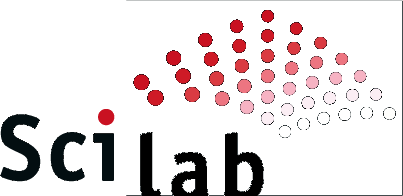
\includegraphics[height=.8cm]{png/logo_scilab}} 
\rotatebox{90}{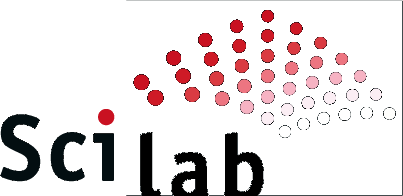
\includegraphics[height=.6cm]{png/logo_scilab}} 
        {\color{violetf}\vrule width 3pt}%
        \hspace{0pt}%must no space.
        \fboxsep=\FrameSep\colorbox{violetc}%
    }%
    \MakeFramed{\hsize #1 \advance\hsize-\width\FrameRestore}%
}%
{\endMakeFramed}%

\newenvironment{pseudo}[1][\hsize]%
{%
    \def\FrameCommand%
    {%
\rotatebox{90}{\textit{\textsf{Pseudo Code}}} 
        {\color{violetf}\vrule width 3pt}%
        \hspace{0pt}%must no space.
        \fboxsep=\FrameSep\colorbox{violetc}%
    }%
    \MakeFramed{\hsize #1 \advance\hsize-\width\FrameRestore}%
}%
{\endMakeFramed}%

\newenvironment{py}[1][\hsize]%
{%
    \def\FrameCommand%
    {%
%\rotatebox{90}{\textit{\textsf{Python}}} 
\rotatebox{90}{
\includegraphics[height=.6cm]{png/logo_python}} 
        {\color{violetf}\vrule width 3pt}%
        \hspace{0pt}%must no space.
        \fboxsep=\FrameSep\colorbox{violetc}%
    }%
    \MakeFramed{\hsize #1 \advance\hsize-\width\FrameRestore}%
}%
{\endMakeFramed}%


\newenvironment{corrige}[1][\hsize]%
{%
    \def\FrameCommand
    {%
\rotatebox{90}{\textit{\textsf{Correction}}} 
        {\color{violetf}\vrule width 3pt}%
        \hspace{0pt}%must no space.
        \fboxsep=\FrameSep\colorbox{violetc}%
    }%
    \MakeFramed{\hsize#1\advance\hsize-\width\FrameRestore}%
}%
{\endMakeFramed}%



\newenvironment{rem}[1][\hsize]%
{%
    \def\FrameCommand
    {%
\rotatebox{90}{\textit{\textsf{Remarque}}} 
        {\color{bleuf}\vrule width 3pt}%
        \hspace{0pt}%must no space.
        \fboxsep=\FrameSep\colorbox{bleuc}%
    }%
    \MakeFramed{\hsize#1\advance\hsize-\width\FrameRestore}%
}%
{\endMakeFramed}%


\newenvironment{savoir}[1][\hsize]%
{%
    \def\FrameCommand
    {%
\rotatebox{90}{\textit{\textsf{Savoir}}} 
        {\color{bleuf}\vrule width 3pt}%
        \hspace{0pt}%must no space.
        \fboxsep=\FrameSep\colorbox{bleuc}%
    }%
    \MakeFramed{\hsize#1\advance\hsize-\width\FrameRestore}%
}%
{\endMakeFramed}%

\newenvironment{prob}[1][\hsize]%
{%
    \def\FrameCommand%
    {%
\rotatebox{90}{\textit{\textsf{ Problématique}}} 
        {\color{rougef}\vrule width 3pt}%
        \hspace{0pt}%must no space.
        \fboxsep=\FrameSep\colorbox{rougec}%
    }%
    \MakeFramed{\hsize#1\advance\hsize-\width\FrameRestore}%
}%
{\endMakeFramed}%

\newenvironment{obj}[1][\hsize]%
{%
    \def\FrameCommand%
    {%
\rotatebox{90}{\textit{\textsf{Objectifs}}} 
        {\color{rougef}\vrule width 3pt}%
        \hspace{0pt}%must no space.
        \fboxsep=\FrameSep\colorbox{rougec}%
    }%
    \MakeFramed{\hsize#1\advance\hsize-\width\FrameRestore}%
}%
{\endMakeFramed}%

\newenvironment{defi}[1][\hsize]%
{%
    \def\FrameCommand%
    {%
\rotatebox{90}{\textit{\textsf{Définition\\}}} 
        {\color{bleuf}\vrule width 3pt}%
        \hspace{0pt}%must no space.
        \fboxsep=\FrameSep\colorbox{bleuc}%
    }%
    \MakeFramed{\hsize#1\advance\hsize-\width\FrameRestore}%
}%
{\endMakeFramed}%


\newenvironment{demo}[1][\hsize]%
{%
    \def\FrameCommand%
    {%
\rotatebox{90}{\textit{\textsf{Démonstration\\}}} 
        {\color{bleuf}\vrule width 3pt}%
        \hspace{0pt}%must no space.
        \fboxsep=\FrameSep\colorbox{bleuc}%
    }%
    \MakeFramed{\hsize#1\advance\hsize-\width\FrameRestore}%
}%
{\endMakeFramed}%


\newenvironment{hypo}[1][\hsize]%
{%
    \def\FrameCommand%
    {%
\rotatebox{90}{\textit{\textsf{Hypothèse\\}}} 
        {\color{bleuf}\vrule width 3pt}%
        \hspace{0pt}%must no space.
        \fboxsep=\FrameSep\colorbox{bleuc}%
    }%
    \MakeFramed{\hsize#1\advance\hsize-\width\FrameRestore}%
}%
{\endMakeFramed}%


\newenvironment{prop}[1][\hsize]%
{%
    \def\FrameCommand%
    {%
\rotatebox{90}{\textit{\textsf{Propriété\\}}} 
        {\color{bleuf}\vrule width 3pt}%
        \hspace{0pt}%must no space.
        \fboxsep=\FrameSep\colorbox{bleuc}%
    }%
    \MakeFramed{\hsize#1\advance\hsize-\width\FrameRestore}%
}%
{\endMakeFramed}%

\newenvironment{props}[1][\hsize]%
{%
    \def\FrameCommand%
    {%
\rotatebox{90}{\textit{\textsf{Propriétés\\}}} 
        {\color{bleuf}\vrule width 3pt}%
        \hspace{0pt}%must no space.
        \fboxsep=\FrameSep\colorbox{bleuc}%
    }%
    \MakeFramed{\hsize#1\advance\hsize-\width\FrameRestore}%
}%
{\endMakeFramed}%

\newenvironment{exemple}[1][\hsize]%
{%
    \def\FrameCommand%
    {%
\rotatebox{90}{\textit{\textsf{Exemple\\}}} 
        {\color{vertf}\vrule width 3pt}%
        \hspace{0pt}%must no space.
        \fboxsep=\FrameSep\colorbox{vertc}%
    }%
    \MakeFramed{\hsize#1\advance\hsize-\width\FrameRestore}%
}%
{\endMakeFramed}%

\newenvironment{resultat}[1][\hsize]%
{%
    \def\FrameCommand%
    {%
\rotatebox{90}{\textit{\textsf{Résultat\\}}} 
        {\color{rougef}\vrule width 3pt}%
        \hspace{0pt}%must no space.
        \fboxsep=\FrameSep\colorbox{rougec}%
    }%
    \MakeFramed{\hsize#1\advance\hsize-\width\FrameRestore}%
}%
{\endMakeFramed}%

\newenvironment{methode}[1][\hsize]%
{%
    \def\FrameCommand%
    {%
\rotatebox{90}{\textit{\textsf{Méthode\\}}} 
        {\color{rougef}\vrule width 3pt}%
        \hspace{0pt}%must no space.
        \fboxsep=\FrameSep\colorbox{rougec}%
    }%
    \MakeFramed{\hsize#1\advance\hsize-\width\FrameRestore}%
}%
{\endMakeFramed}%

\newenvironment{theo}[1][\hsize]%
{%
    \def\FrameCommand%
    {%
\rotatebox{90}{\textit{\textsf{Théorème\\}}} 
        {\color{rougef}\vrule width 3pt}%
        \hspace{0pt}%must no space.
        \fboxsep=\FrameSep\colorbox{rougec}%
    }%
    \MakeFramed{\hsize#1\advance\hsize-\width\FrameRestore}%
}%
{\endMakeFramed}%

\newenvironment{warn}[1][\hsize]%
{%
    \def\FrameCommand%
    {%
\rotatebox{90}{\textit{\textsf{Attention\\}}} 
        {\color{rougef}\vrule width 3pt}%
        \hspace{0pt}%must no space.
        \fboxsep=\FrameSep\colorbox{rougec}%
    }%
    \MakeFramed{\hsize#1\advance\hsize-\width\FrameRestore}%
}%
{\endMakeFramed}%

% \usepackage{pstricks}
%\usepackage{minitoc}
% \setcounter{minitocdepth}{4}

\setcounter{tocdepth}{2}

% \mtcselectlanguage{french} 

%\usepackage{draftcopy}% "Brouillon"
% \usepackage{floatflt}
\usepackage{psfrag}
%\usepackage{listings} % Permet d'insérer du code de programmation
\renewcommand{\baselinestretch}{1.2}

% Changer la numérotation des figures :
% ------------------------------------
% \makeatletter
% \renewcommand{\thefigure}{\ifnum \c@section>\z@ \thesection.\fi
%  \@arabic\c@figure}
% \@addtoreset{figure}{section}
% \makeatother
 


%%%%%%%%%%%%
% Définition des vecteurs %
%%%%%%%%%%%%
 \newcommand{\vect}[1]{\overrightarrow{#1}}

%%%%%%%%%%%%
% Définition des torseusr %
%%%%%%%%%%%%

 \newcommand{\torseur}[1]{%
\left\{{#1}\right\}
}

\newcommand{\torseurcin}[3]{%
\left\{\mathcal{#1} \left(#2/#3 \right) \right\}
}

\newcommand{\torseurstat}[3]{%
\left\{\mathcal{#1} \left(#2\rightarrow #3 \right) \right\}
}

 \newcommand{\torseurc}[8]{%
%\left\{#1 \right\}=
\left\{
{#1}
\right\}
 = 
\left\{%
\begin{array}{cc}%
{#2} & {#5}\\%
{#3} & {#6}\\%
{#4} & {#7}\\%
\end{array}%
\right\}_{#8}%
}

 \newcommand{\torseurcol}[7]{
\left\{%
\begin{array}{cc}%
{#1} & {#4}\\%
{#2} & {#5}\\%
{#3} & {#6}\\%
\end{array}%
\right\}_{#7}%
}

 \newcommand{\torseurl}[3]{%
%\left\{\mathcal{#1}\right\}_{#2}=%
\left\{%
\begin{array}{l}%
{#1} \\%
{#2} %
\end{array}%
\right\}_{#3}%
}

 \newcommand{\vectv}[3]{%
\vect{V\left( {#1} \in {#2}/{#3}\right)}
}


\newcommand{\vectf}[2]{%
\vect{R\left( {#1} \rightarrow {#2}\right)}
}

\newcommand{\vectm}[3]{%
\vect{\mathcal{M}\left( {#1}, {#2} \rightarrow {#3}\right)}
}


 \newcommand{\vectg}[3]{%
\vect{\Gamma \left( {#1} \in {#2}/{#3}\right)}
}

 \newcommand{\vecto}[2]{%
\vect{\Omega\left( {#1}/{#2}\right)}
}
% }$$\left\{\mathcal{#1} \right\}_{#2} =%
% \left\{%
% \begin{array}{c}%
%  #3 \\%
%  #4 %
% \end{array}%
% \right\}_{#5}}

%  ------------------------------------------
% | Modification du formatage des sections : | 
%  ------------------------------------------

% Grands titres :
% ---------------

\newcommand{\titre}[1]{%
\begin{center}
      \bigskip
      \rule{\textwidth}{1pt}
      \par\vspace{0.1cm}
      
      \textbf{\large #1}
      \par\rule{\textwidth}{1pt}
    \end{center}
    \bigskip
  }

% Supprime le numéro du chapitre dans la numérotation des sections:
% -----------------------------------------------------------------
\makeatletter
\renewcommand{\thesection}{\@arabic\c@section}
\makeatother


% \titleformat{\chapter}[display]
% {\normalfont\Large\filcenter}
% {}
% {1pc}
% {\titlerule[1pt]
%   \vspace{1pc}%
%   \Huge}[\vspace{1ex}%
% \titlerule]


%%%% Chapitres Comme PY Pechard %%%%%%%%%
% numéro du chapitre
\DeclareFixedFont{\chapnumfont}{OT1}{phv}{b}{n}{80pt}
% pour le mot « Chapitre »
\DeclareFixedFont{\chapchapfont}{OT1}{phv}{m}{it}{40pt}
% pour le titre
\DeclareFixedFont{\chaptitfont}{T1}{phv}{b}{n}{25pt}

\definecolor{gris}{gray}{0.75}
\titleformat{\chapter}[display]%
	{\sffamily}%
	{\filleft\chapchapfont\color{gris}\chaptertitlename\
	\\
	\vspace{12pt}
	\chapnumfont\thechapter}%
	{16pt}%
	{\filleft\chaptitfont}%
	[\vspace{6pt}\titlerule\titlerule\titlerule]

%%%%  Fin Chapitres Comme PY Pechard %%%%%%%%%


% Section, subsection, subsubsection sans serifs :
% % ----------------------------------------------

% \makeatletter
% \renewcommand{\section}{\@startsection{section}{0}{0mm}%
% {\baselineskip}{.3\baselineskip}%
% {\normalfont\sffamily\Large\textbf}}%
% \makeatother

\makeatletter
\renewcommand{\@seccntformat}[1]{{\textcolor{bleu}{\csname
the#1\endcsname}\hspace{0.5em}}}
\makeatother

\makeatletter
\renewcommand{\section}{\@startsection{section}{1}{\z@}%
                       {-4ex \@plus -1ex \@minus -.4ex}%
                       {1ex \@plus.2ex }%
                       {\normalfont\Large\sffamily\bfseries}}%
\makeatother
 
\makeatletter
\renewcommand{\subsection}{\@startsection {subsection}{2}{\z@}
                          {-3ex \@plus -0.1ex \@minus -.4ex}%
                          {0.5ex \@plus.2ex }%
                          {\normalfont\large\sffamily\bfseries}}
\makeatother
 
\makeatletter
\renewcommand{\subsubsection}{\@startsection {subsubsection}{3}{\z@}
                          {-2ex \@plus -0.1ex \@minus -.2ex}%
                          {0.2ex \@plus.2ex }%
                          {\normalfont\large\sffamily\bfseries}}
\makeatother
 
\makeatletter             
\renewcommand{\paragraph}{\@startsection{paragraph}{4}{\z@}%
                                    {-2ex \@plus-.2ex \@minus .2ex}%
                                    {0.1ex}%               
{\normalfont\sffamily\bfseries}}
\makeatother
 

\makeatletter             
\renewcommand{\subparagraph}{\@startsection{subparagraph}{5}{\z@}%
                                    {-2ex \@plus-.2ex \@minus .2ex}%
                                    {0.1ex}%               
{\normalfont\bfseries Question }}
\makeatother

\renewcommand{\thesubparagraph}{\arabic{subparagraph}} 
\makeatletter

\setcounter{secnumdepth}{5}
%\renewcommand{\subparagraph}{\@startsection{subparagraph}{5}{\z@}%
%                                       {-2ex \@plus-.1ex \@minus .2ex}%
%                                       {0.1ex}%
%				    {\normalfont\normalsize\sffamily\bfseries}}
%\makeatletter
% \makeatletter
% \renewcommand{\subsection}{\@startsection{subsection}{1}{2mm}%
% {\baselineskip}{.3\baselineskip}%
% {\normalfont\sffamily\large\textbf}}%
% \makeatother
% 
% \makeatletter
% \renewcommand{\subsubsection}{\@startsection{subsubsection}{2}{4mm}%
% {\baselineskip}{.15\baselineskip}%
% {\normalfont\sffamily\large\textbf}}%
% \makeatother
% 
% \makeatletter
% \renewcommand{\paragraph}{\@startsection{paragraph}{3}{6mm}%
% {\baselineskip}{.15\baselineskip}%
% {\normalfont\sffamily\large\textbf}}%
% \makeatother
 



%  --------
% | Marges |
%  --------


% \setmarginsrb{2.5cm}{1.5cm}{2.5cm}{2cm}{1cm}{1cm}{1cm}{1cm}
\setmarginsrb{1.5cm}{1cm}{1cm}{1.5cm}{1cm}{1cm}{1cm}{1cm}

% Changer les marges localement :
% -----------------------------
\newenvironment{changemargin}[2]{\begin{list}{}{%
\setlength{\topsep}{0pt}%
\setlength{\leftmargin}{0pt}%
\setlength{\rightmargin}{0pt}%
\setlength{\listparindent}{\parindent}%
\setlength{\itemindent}{\parindent}%
\setlength{\parsep}{0pt plus 1pt}%
\addtolength{\leftmargin}{#1}%
\addtolength{\rightmargin}{#2}%
}\item }{\end{list}}



\usepackage{pst-solides3d}
\usepackage{titletoc}
\titlecontents{chapter}[+3pc]
  {\addvspace{10pt}\sffamily\bfseries}
{\contentslabel[{\pscirclebox[fillstyle=solid,fillcolor=gray!25,
linecolor=gray!25,framesep=4pt]{\textcolor{white}{\thecontentslabel}}}]{2.5pc}}
  {}
  {\dotfill \normalfont\thecontentspage\ }

\titlecontents{section}[3pc]
  {\addvspace{2pt}\sffamily}
  {\contentslabel[\thecontentslabel]{1.8pc}}
  {}
  {\dotfill \normalfont\thecontentspage\ }

\titlecontents{subsection}[5pc]
  {\addvspace{2pt}\sffamily}
  {\contentslabel[\thecontentslabel]{1.8pc}}
  {}
  {\dotfill \normalfont\thecontentspage\ }

\titlecontents{subsubsection}[8pc]
  {\addvspace{2pt}\sffamily}
  {\contentslabel[\thecontentslabel]{3pc}}
  {}
  {\dotfill \normalfont\thecontentspage\ }
%{\;\titlerule\;\normalfont\thecontentspage\ }

\titlecontents{paragraph}[9pc]
  {\addvspace{2pt}\sffamily}
  {\contentslabel[\thecontentslabel]{3.5pc}}
  {}
  {\dotfill \normalfont\thecontentspage\ }




%Si le boolen xp est vrai : compilation pour xabi
%Sinon compilation Damien
\newboolean{xp}
\setboolean{xp}{true}

\newboolean{prof}
\setboolean{prof}{false}

\def\xxtitre{\ifthenelse{\boolean{xp}}{
CI 3 -- CIN : Étude du comportement cinématique des systèmes}{
}}

\def\xxsoustitre{\ifthenelse{\boolean{xp}}{
Devoir Maison 6}{
}}


\def\xxauteur{\ifthenelse{\boolean{xp}}{
\noindent 2013 -- 2014 \\
Xavier \textsc{Pessoles}}{
}}


\def\xxpied{\ifthenelse{\boolean{xp}}{
CI 3 : CIN\\
DM 6 : \ifthenelse{\boolean{prof}}{P}{E}%
}{
}}

\usepackage[%
    pdftitle={CIN},
    pdfauthor={Xavier Pessoles},
    colorlinks=true,
    linkcolor=blue,
    citecolor=magenta]{hyperref}



\usepackage{pifont}
\sloppy
\hyphenpenalty 10000


\begin{document}






% \makeatletter \let\ps@plain\ps@empty \makeatother
%% DEBUT DU DOCUMENT
%% =================




%------------- En tetes et Pieds de Pages ------------


\pagestyle{fancy}
\ifthenelse{\boolean{xp}}{%
\renewcommand{\headrulewidth}{0pt}}{%
\renewcommand{\headrulewidth}{0.2pt}} %pour mettre le trait en haut
%\renewcommand{\headrulewidth}{0.2pt}

\fancyhead{}
\fancyhead[L]{%
\ifthenelse{\boolean{xp}}{%
\noindent\begin{minipage}[c]{2.6cm}%

\includegraphics[width=2cm]{png/logo_ptsi.png}%
\end{minipage}%
}{%
\footnotesize{\textit{\textsf{Lycée François Premier}}}
}}

\ifthenelse{\boolean{xp}}{%
\fancyhead[C]{\rule{12cm}{.5pt}}}{
}


\fancyhead[R]{%
\noindent\begin{minipage}[c]{3cm}
\begin{flushright}
\footnotesize{\textit{\textsf{Sciences Industrielles \\ de l'ingénieur}}}%
\end{flushright}
\end{minipage}
}


\ifthenelse{\boolean{xp}}{%
\fancyhead[C]{\rule{12cm}{.5pt}}}{
}

\renewcommand{\footrulewidth}{0.2pt}

\fancyfoot[C]{\footnotesize{\bfseries \thepage}}
\fancyfoot[L]{%
\begin{minipage}[c]{.2\linewidth}
\noindent\footnotesize{{\xxauteur}}
\end{minipage}
\ifthenelse{\boolean{xp}}{}{%
\begin{minipage}[c]{.15\linewidth}

\includegraphics[width=2cm]{png/logoCC.png}
\end{minipage}}
}


\fancyfoot[R]{\footnotesize{\xxpied}}



\begin{center}
 \Large\textsc{\xxtitre}
\end{center}

\begin{center}
 \large\textsc{\xxsoustitre}
\end{center}

%\vspace{.5cm}




%

\section{Presse Cisaille à Bac CVB 1000 T}

\ifthenelse{\boolean{prof}}{\textit{{Activité proposée par Pierre Debout}}}{}

\subsection{Mise en situation}
\ifthenelse{\boolean{prof}}{}{
La société COPEX, installée à Lanester (56 Morbihan) est spécialisée dans les machines et leurs applications à l’environnement. Elle conçoit et fabrique, en particulier du matériel permettant de compacter des déchets de différentes natures, afin d’éventuellement les retraiter ou de les stocker. 

L’étude proposée porte sur une Presse / Cisaille type CVB 1 000 T (Cisaille Verticale à Bac de 1 000 tonnes) destinée à traiter de la ferraille de toute sorte. En fonction des matériaux récupérés, elle permet le compactage sous forme de paquet ou le cisaillage afin de diminuer les volumes lors du transport avant retraitement ou stockage final.

\begin{center}
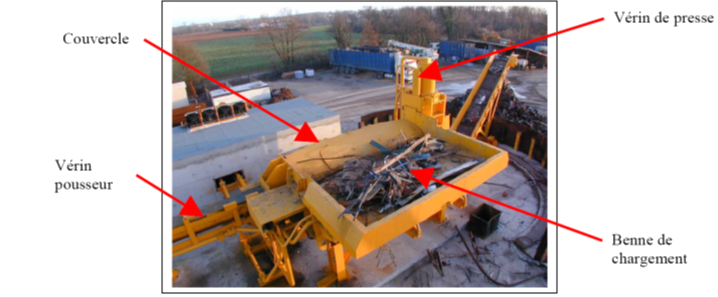
\includegraphics[width=.75\textwidth]{png/fig1}
\end{center}

La machine permet deux processus différents : 
\begin{itemize}
\item la réduction de volume par compactage pour l’obtention de paquet; 

\begin{center}
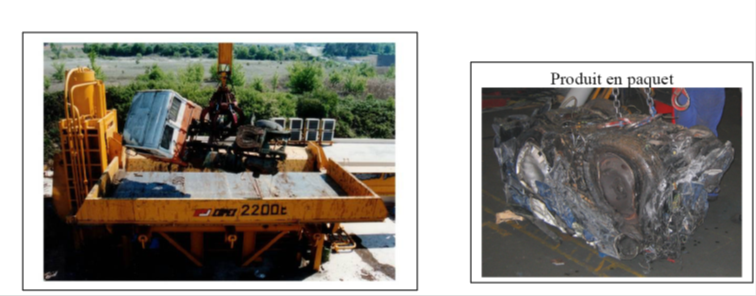
\includegraphics[width=.75\textwidth]{png/fig2}
\end{center}

\item la réduction de volume par compactage et cisaillage sous forme de bouts de métal découpés à des longueurs variables de 30 à 95 cm. 
\end{itemize}


\begin{center}
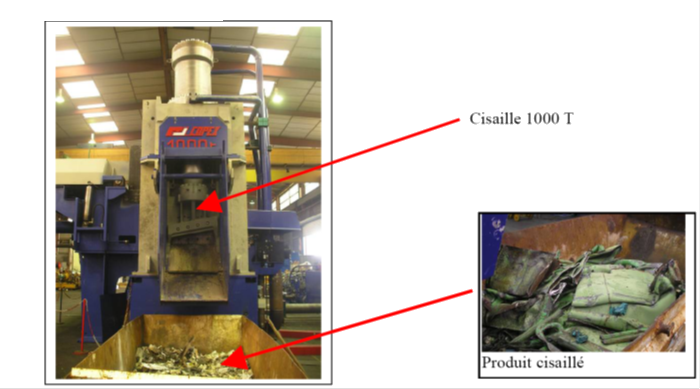
\includegraphics[width=.75\textwidth]{png/fig3}
\end{center}
}

\subsection{Fonctionnement}
\ifthenelse{\boolean{prof}}{}{
Vue schématique de la machine, de ses mouvements et des détecteurs associés :

\begin{center}
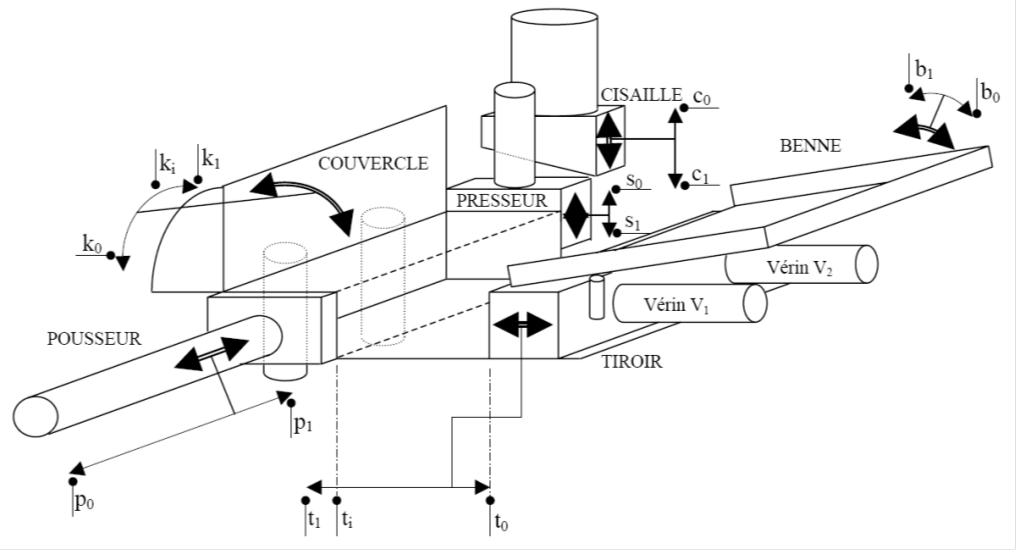
\includegraphics[width=.75\textwidth]{png/fig4}
\end{center}


Le fonctionnement général de la cisaille est le suivant : 
\begin{itemize}
\item la machine est prête pour un chargement et le système est en position initiale;
\item le compactage est effectué grâce à quatre actionneurs, pilotés manuellement par l’utilisateur: 
\begin{itemize}
\item basculement de la « Benne » pour déchargement de la matière dans la caisse de compression ;
\item retour « Benne » à l’horizontale ;
\item compression latérale par l’avance partielle du piston « Tiroir », animé par 2 vérins $V_1$ et $V_2$;
\item recul du « Tiroir »;
\item compression supérieure par la fermeture partielle du « Couvercle », animé par 2 vérins;
\item ouverture du « Couvercle »;
\item fermeture du « Couvercle » en position horizontale;
\item fermeture du « Tiroir » en position coïncidente à la largeur du « Pousseur »;
\item compression longitudinale par le piston « Pousseur ».
\end{itemize}
\end{itemize}

Le compactage étant terminé, deux modes automatisés sont disponibles : 
\begin{itemize}
\item mode paquet qui permet l’évacuation du bloc de métal ;
\begin{itemize}
\item montée de la « Cisaille » ;
\item montée de la Porte (« Presseur ») ;
\item avance du paquet poussé par le piston « Pousseur » ; 
\end{itemize}
\item mode cisaille qui permet le cisaillage et l’évacuation des morceaux de ferraille. 
Ce cycle se répète $N$ fois en fonction des longueurs $L$ souhaitées par l’opérateur pour les bouts de ferrailles. Chaque cycle est réalisé de la façon suivante : 
\begin{itemize}
\item montée de la « Cisaille » ;
\item montée de la Porte (« Presseur ») ;
\item avance de la matière par le piston « Pousseur » jusqu’à atteindre la position fonction de la longueur des bouts de ferraille souhaitée ;
\item descente du « Presseur » jusqu’à atteindre une position intermédiaire ;
\item descente de la « Cisaille » et découpe de la matière.
\end{itemize}
\end{itemize}
Les informations issues des capteurs de fin de course $c_i$, $k_i$, $s_i$, parviennent à l’unité de commande qui pilote les actionneurs du pousseur, du presseur et de la cisaille.
}

\subsection{Analyse du système}


\subparagraph{}
\textit{Proposer 3 exigences associées pour chacune à un critère et un niveau qui vous semble crédible.}
\ifthenelse{\boolean{prof}}{
\begin{corrige}
\begin{center}
\begin{tabular}{|l|l|l|}
\hline 
Exigences & Critère & Niveau \\
\hline 
\hline 
Compacter des matériaux métalliques & Force de coupe & Equivalent à $1\; 000$ tonnes.\\
\hline 
Cisailler la ferraille à longueur variable & Longueur des morceaux & 30 à 95 cm \\
\hline
Compacter rapidement une grande quantité de ferraille & Cadence maximale & 30 tonnes à l'heure \\
\hline
\end{tabular}
\end{center}
\end{corrige}}{}

\ifthenelse{\boolean{prof}}{}{
Le diagramme de définition des blocs de la Presse / Cisaille type CVB 1 000 T est présenté ci-dessous :
\begin{itemize}
\item la centrale hydraulique fournit l’énergie hydraulique au système;
\item l’unité de commande permet de traiter les informations provenant des différents capteurs et d’exécuter le programme gérant les opérations automatisées;
\item le pupitre de contrôle est l’interface homme machine permettant à l’opérateur de contrôler la machine.
\end{itemize}


\begin{center}
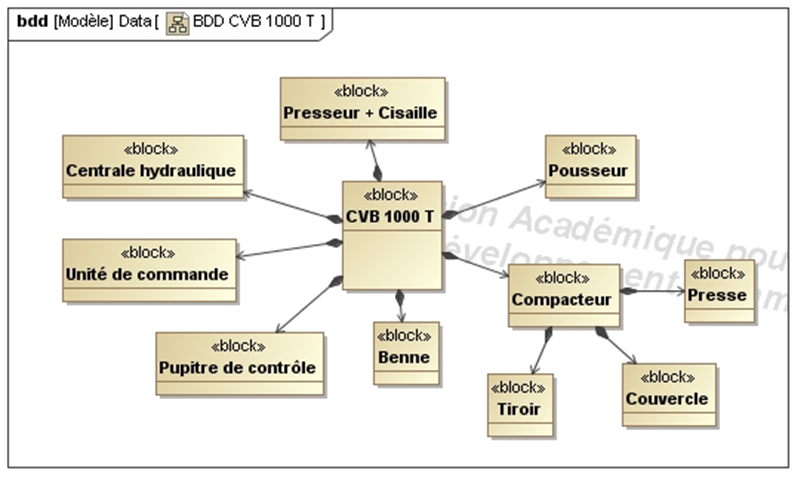
\includegraphics[width=.75\textwidth]{png/fig5}
\end{center}
}

\subparagraph{}
\textit{Compléter le diagramme des blocs internes sur le document réponse en nommant et en distinguant les flux (matière en bleu, énergie en rouge, information en vert).}
\ifthenelse{\boolean{prof}}{
\begin{corrige}

\begin{center}
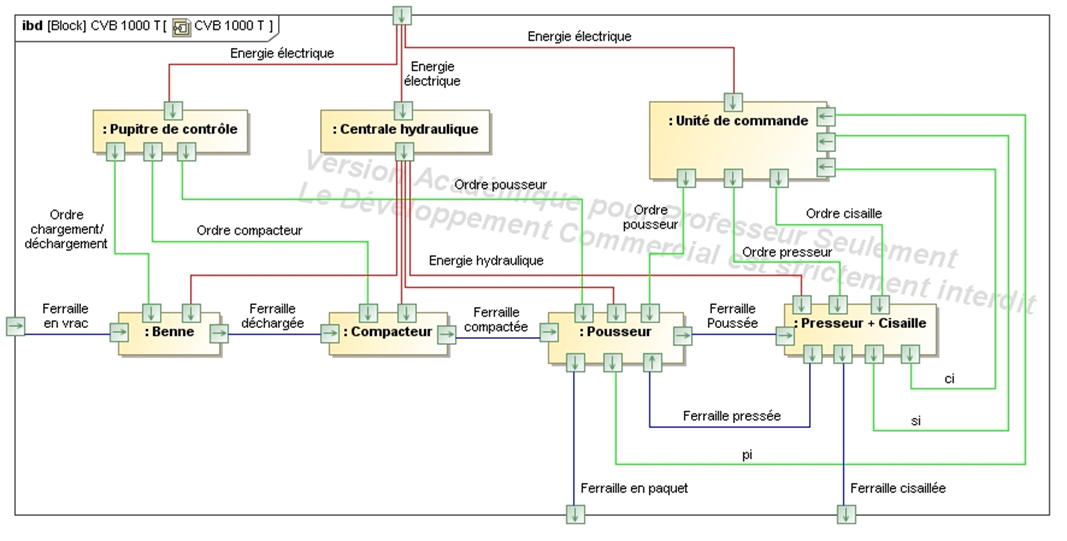
\includegraphics[width=.95\textwidth]{png/q2}
\end{center}

\end{corrige}}{}


\subsection{Étude de l'asservissement}

\ifthenelse{\boolean{prof}}{}{
Le déplacement en translation du tiroir 1 est assuré par deux vérins hydrauliques V1 et V2 asservis en position. Les deux vérins hydrauliques sont montés en portique en deux points d’ancrage (en parallèle) sur le tiroir. Chaque vérin du type « mesure en position intégrée » (détecteur inductif intégré dans la tige du vérin, résolution $\pm \; 0,1\;mm$) est piloté par un servodistributeur. Les commandes des deux vérins sont synchronisées. 

On isole l’un des vérins. Le comportement d’un vérin peut alors être modélisé à partir du modèle de structure ci-dessous et du paramétrage qui lui est associé. 


\begin{center}
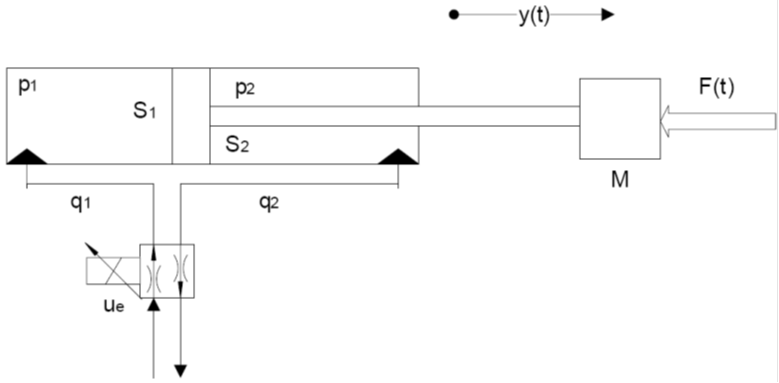
\includegraphics[width=.75\textwidth]{png/fig6}
\end{center}

L’ensemble formé par le tiroir et la tige du piston du vérin, est appelé « équipage mobile ». Sa position notée $y(t)$ est fonction du débit d’huile, noté $q_1(t)$, à l’entrée de la chambre d’admission du vérin. 

L’effort variable dû à la ferraille est noté $F(t)$.
On se place dans l’hypothèse de petit déplacement autour d’un point de fonctionnement (position particulière d’équilibre). Le système peut donc être considéré comme linéaire, continu et invariant. $u_e(t)$ est la tension de commande variable du servodistributeur.

On donne : 
\begin{itemize}
\item $M = 10^4\;kg$ : masse de l’équipage mobile ; 
\item $f = 3\cdot10^6\; N/(m/s)$ : résistance due aux frottements visqueux ; 
\item $K = 2,5\cdot10^7\; N/m$ : raideur hydraulique du vérin ; 
\item $S_1 = 5\cdot10^{-2}\; m^2$ : surface du piston de la chambre d’admission. 
\end{itemize}
}

\subsubsection{Modélisation de l'équipage mobile}
\ifthenelse{\boolean{prof}}{}{
L’équation temporelle donnant le déplacement $y_1(t)$ en fonction du débit $q_1(t)$ pour un effort $F(t)$ nul est telle que : 
$$
M\dfrac{d^2 y_1(t)}{dt^2}= K\int\limits_{0}^{t} \dfrac{q_1(\tau)}{S_1}d\tau - Ky_1(t)-f\dfrac{dy_1(t)}{dt}
$$
 
L’équation temporelle donnant le déplacement $y_2(t)$ en fonction de l’effort $F(t)$ pour un débit $q_1(t)$ nul est telle que : 
$$
M\dfrac{d^2 y_1(t)}{dt^2}=-Ky_2(t) - f \dfrac{dy_2(t)}{dt}+F(t)
$$
Le déplacement total pour l’équipage mobile du vérin $V_1$ est alors $y(t)=y_1 (t)+y_2 (t)$.
}


\subparagraph{}
\textit{En supposant que les conditions initiales sont nulles, donner dans le domaine de Laplace et sous forme canonique : 
\begin{itemize}
\item la fonction de transfert $H_1 (p)=\dfrac{Y_1 (p)}{Q_1 (p)}$ pour $F(p)$ (image de l’effort $F(t)$) nul ;
\item la fonction de transfert  $H_2 (p)=\dfrac{Y_2 (p)}{F(p)}$ pour $Q_1(p)$ (image du débit $q_1(t)$) nul. 
\end{itemize}
On donnera les formes littérales puis numériques.
}

\ifthenelse{\boolean{prof}}{
\begin{corrige}
D'une part, 
$$
Mp^2 Y_1(p)= \dfrac{KQ_1(p)}{S_1p} - KY_1(p)-fpY_1(p) \Longleftrightarrow 
H_1 (p)=\dfrac{Y_1 (p)}{Q_1 (p)}=\dfrac{\dfrac{K}{S_1p}}{Mp^2  +fp+ K}
=\dfrac{1}{S_1}\dfrac{1}{p\left( \dfrac{M}{K}p^2  +\dfrac{f}{K}p+1\right)}
$$

D'autre part, 
$$
Mp^2 Y_1(p) =-KY_2(p) - f pY_2(p)+F(p) \Longleftrightarrow 
H_2 (p)=\dfrac{Y_2 (p)}{F(p)} = \dfrac{1}{Mp^2+  f p + K} = 
\dfrac{\dfrac{1}{K}}{\dfrac{M}{K}p^2+  \dfrac{f}{K}p + 1} 
$$

En réalisant l'application numérique, on a : 
$$
H_1 (p)=\dfrac{20}{p\left( 4\cdot 10^{-4}\cdot p^2  +0,12\cdot p+1\right)}
\quad
H_2 (p)=\dfrac{4\cdot 10^{-8}}{ 4\cdot 10^{-4}\cdot p^2  +0,12\cdot p+1} 
$$
\end{corrige}}{}


\subparagraph{}
\textit{En appliquant le principe de superposition, donner l’équation, dans le domaine de Laplace, liant $Y(p)$ à $Q_1(p)$ et à $F(p)$.}
\ifthenelse{\boolean{prof}}{
\begin{corrige}

En utilisant le théorème de superposition, on a :

$$
Y(p)=H_1(p) Q_1(p) + F(p) Y_2(p)
$$

\end{corrige}}{}


\subparagraph{}
\textit{Compléter sur le document réponse le schéma bloc permettant de définir la modélisation de l’« équipage mobile ». Préciser les unités des grandeurs physiques véhiculées.}
\ifthenelse{\boolean{prof}}{
\begin{corrige}

\begin{center}
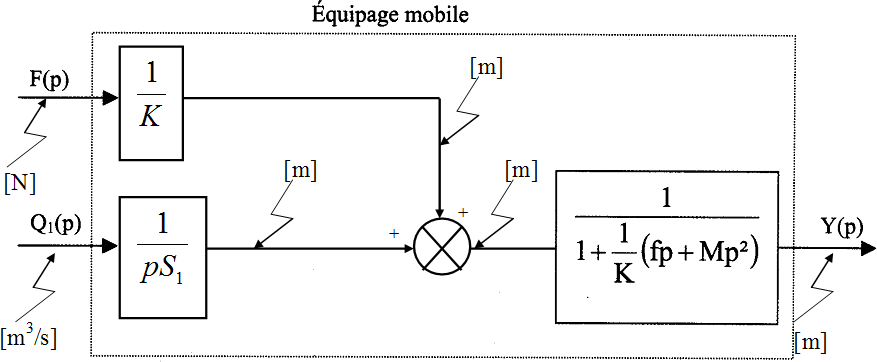
\includegraphics[width=.75\textwidth]{png/q5}
\end{center}

\end{corrige}}{}

\subsubsection{Modélisation générale du fonctionnement de l'ensemble vérin et distribution}

\ifthenelse{\boolean{prof}}{}{
Pour étudier l’influence du débit, on néglige la contribution de l’effort $F(t)$. La fonction de transfert déplacement / débit est alors : 
$$
G(p)=\dfrac{Y(p)}{Q_1(p)}=\dfrac{1}{pS_1\left(1+\dfrac{1}{K}\left( fp+Mp^2\right) \right)}
$$

On admettra que ce résultat est généralisable pour toute position de la tige de vérin. 

Le servodistributeur proportionnel délivre un débit d’huile $q_1(t)$ proportionnel à sa tension de commande $u_e(t)$ tel que : $q_1 (t)=K_e u_e(t)$ avec $K_e = 2\cdot 10^{-4} m^3/(s\cdot V)$.

Le détecteur de position délivre une tension $u_s(t)$ proportionnelle à la position $y(t)$ du tiroir telle que :  $u_S (t)=K_c \cdot y(t)$ avec $K_c = 10^3\; V/m$. 
}

\subparagraph{}
\textit{En déduire la fonction de transfert en boucle ouverte du système tiroir-vérin-distribution dont la transmittance est : $F_{BO} (p)=\dfrac{U_s (p)}{U_e (p)}$. On donnera la forme littérale puis numérique.}
\ifthenelse{\boolean{prof}}{
\begin{corrige}

On a :

$$
\dfrac{U_S(p)}{U_e(p)} = K_C K_e G(p) = \dfrac{K_C K_e / S_1}{p\left( \dfrac{M}{K}p^2  +\dfrac{f}{K}p+1\right)}
$$

Après application numérique : 

$$
\dfrac{U_S(p)}{U_e(p)} = \dfrac{4}{p\left(4\cdot 10^{-4}\cdot p^2  +0,12\cdot p+1\right)}
$$

\end{corrige}}{}

\ifthenelse{\boolean{prof}}{}{
Quel que soit le résultat de la question précédente, on considère par la suite que la fonction de transfert en boucle ouverte peut se mettre sous la forme : 
$$
F_{BO}(p)=\dfrac{U_s (p)}{U_e (p)}=\dfrac{4}{p\left(1+0,12p+0,0004p^2 \right)}
$$

%\subparagraph{}
%\textit{Exprimer $F_{BO}(p)$ comme un produit de 2 fonctions de transfert fondamentales. Définir puis calculer les caractéristiques de ces fonctions nécessaires au tracé du diagramme de Bode. En utilisant plusieurs couleurs, tracer sur le document réponse les diagrammes de Bode asymptotique des 2 fonctions choisies et de $F_{BO}(j\omega)$.}
%\ifthenelse{\boolean{prof}}{
%\begin{corrige}
%\end{corrige}}{}

Pour boucler le système : 
\begin{itemize}
\item le signal de la commande du distributeur proportionnel $u_e(t)$ est élaboré à partir : 
\begin{itemize}
\item d’un élément permettant de comparer $u_s(t)$ à la tension de consigne $u_c(t)$;
\item d’un amplificateur de gain $A$. 
\end{itemize}
\item le signal de tension de consigne $u_c(t)$ est élaboré à partir de la consigne de position $y_c(t)$ et d’un potentiomètre modélisable par un gain pur identique à $K_c$. 
\end{itemize}
}

\subparagraph{}
\textit{Compléter le schéma bloc permettant de définir le système tiroir-vérin-distribution, son contrôle et sa commande dont la fonction de transfert en boucle fermée est : $\dfrac{Y(p)}{Y_c (p)}$.}
\ifthenelse{\boolean{prof}}{
\begin{corrige}
\begin{center}
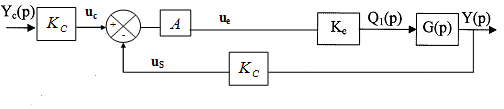
\includegraphics[width=.75\textwidth]{png/q8}
\end{center}

\end{corrige}}{}


\subparagraph{}
\textit{Calculer la fonction de transfert en boucle fermée sous sa forme canonique : $\dfrac{Y(p)}{Y_c (p)}$ en fonction des différents coefficients littéraux caractérisant le système. Effectuer l’application numérique pour $A=1$.}
\ifthenelse{\boolean{prof}}{
\begin{corrige}
$$
\dfrac{Y(p)}{Y_C(p)} 
= \dfrac{AK_CK_e G(p)}{1+AK_CK_e G(p)} 
= \dfrac{\dfrac{A K_C K_e / S_1}{p\left( \dfrac{M}{K}p^2  +\dfrac{f}{K}p+1\right)}}{1+\dfrac{A K_C K_e / S_1}{p\left( \dfrac{M}{K}p^2  +\dfrac{f}{K}p+1\right)}}
= \dfrac{A K_C K_e / S_1}{A K_C K_e / S_1 + p\left( \dfrac{M}{K}p^2  +\dfrac{f}{K}p+1\right)}
$$

$$
\dfrac{Y(p)}{Y_C(p)} 
= \dfrac{1}{1 + \dfrac{S_1}{A K_C K_e}p  
+\dfrac{S_1}{A K_C K_e}\dfrac{f}{K}p^2
+ \dfrac{S_1}{A K_C K_e} \dfrac{M}{K}p^3 }
$$

Application numérique : 
$$
\dfrac{Y(p)}{Y_C(p)} =
\dfrac{1}{1+0,25p + 0,03 p^2 + 10^{-4}p^3}
$$

\end{corrige}}{}

\ifthenelse{\boolean{prof}}{}{
On considère par la suite que la fonction de transfert en boucle fermée peut se mettre sous la forme : 
$$\dfrac{Y(p)}{Y_c (p)}=\dfrac{1}{1+0,25p+0,03p^2}$$
}


\subparagraph{}
\textit{Calculer les caractéristiques de cette transmittance. Que pensez-vous de la valeur du coefficient d’amortissement vis-à-vis du critère de rapidité ?}
\ifthenelse{\boolean{prof}}{
\begin{corrige}
Le système est un système du second ordre de gain statique $K = 1$, de pulsation $\omega_0 = 6\; rad/s$ et d'amortissement $\xi = 0,75$. 

Dans ce cas $\xi$ est légèrement supérieur à 0,7. Il y aura donc un léger dépassement et le temps de réponse sera calculé sur la montée de la réponse temporelle. 

\end{corrige}}{}

\subsubsection{Étude en position}
Le système est alors soumis à une consigne $y_c(t) = u(t)$ où $u(t)$ désigne l'échelon défini par : 
\begin{itemize}
\item $u(t) = 0$ si $t < 0$ ;
\item $u(t) = 100\; mm$ si $t > 0$.
\end{itemize}




\subparagraph{}
\textit{Tracer l’allure de la courbe de la réponse du système à ce signal sur la figure du document réponse. On veut voir apparaître :
\begin{itemize}
\item la pente à l’origine; 
\item les éventuels dépassements (on peut utiliser l’annexe); 
\item la courbe en régime permanent. 
\end{itemize}}
\ifthenelse{\boolean{prof}}{
\begin{corrige}
\begin{center}
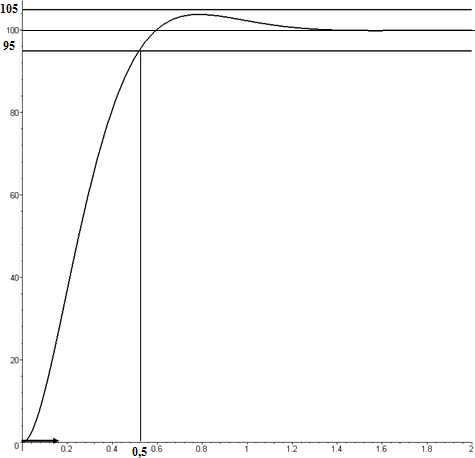
\includegraphics[width=.5\textwidth]{png/q11}
\end{center}
\end{corrige}}{}


\subparagraph{}
\textit{Calculer analytiquement puis numériquement l’écart statique (ou erreur de position). 
Que peut-on en conclure vis-à-vis de la précision ?}
\ifthenelse{\boolean{prof}}{
\begin{corrige}
$$
\varepsilon_S  
= \lim\limits_{t\to \infty} \left(y(t)-y_c(t) \right)
= \lim\limits_{p\to 0} p \left(Y(p)-Y_c(p) \right)
= \lim\limits_{p\to 0} p \dfrac{100}{p}(1-1)
= 0\; mm
$$

L'asservissement est donc précis. 
\end{corrige}}{}


Dans la réalité le servodistributeur proportionnel délivre un débit d’huile $q_1(t)$ avec un retard de $\tau = 0,1\;s$ et un gain $K_e = 2\cdot 10^{-4} m^3/(s\cdot V)$ qui équivaut à un premier ordre. 

\subparagraph{}
\textit{Calculer la nouvelle fonction de transfert en boucle fermée sous sa forme canonique : $\dfrac{Y(p)}{Y_c (p)}$ en fonction des différents coefficients littéraux caractérisant le système. Effectuer l’application numérique pour $A=1$.}
\ifthenelse{\boolean{prof}}{
\begin{corrige}
$$
\dfrac{Q_1(p)}{U_e(p)} = \dfrac{K_e}{1+\tau p} = \dfrac{2\cdot 10^{-4}}{1+0,1 p}
$$

$$
\dfrac{Y(p)}{Y_c(p)}
=\dfrac{AK_C \dfrac{K_e}{1+\tau p}G(p)}{1+AK_C \dfrac{K_e}{1+\tau p}G(p)}
= \dfrac{
\dfrac{AK_CK_e/S_1}{p\left( 1 +\tau p\right) \left( \dfrac{M}{K}p^2 + \dfrac{f}{K}p + 1\right)}
}{1+\dfrac{AK_CK_e/S_1}{p\left( 1 +\tau p\right) \left( \dfrac{M}{K}p^2 + \dfrac{f}{K}p + 1\right)}}
=
\dfrac{AK_CK_e/S_1}{p\left( 1 +\tau p\right) \left( \dfrac{M}{K}p^2 + \dfrac{f}{K}p + 1\right)+AK_CK_e/S_1}
$$

$$
\dfrac{Y(p)}{Y_c(p)} = \dfrac{1}{
1+\dfrac{S_1}{AK_CK_e}p + \left(\dfrac{f}{K} +\tau \right)\dfrac{S_1}{AK_CK_e}p^2
+\left(\dfrac{M+\tau f}{K}\right)\dfrac{S_1}{AK_CK_e}p^3
+\dfrac{M\tau }{K}\dfrac{S_1}{AK_CK_e}p^4
}$$

$$
\dfrac{Y(p)}{Y_c(p)} = 
\dfrac{1}{1+0,25 p + 0,055 p^2 + 3,1\cdot 10^{-3} p^3 + 10^{-5}p^4}
$$
\end{corrige}}{}


\subparagraph{}
\textit{D’après le tracé de la réponse à un échelon d’amplitude $100\;mm$ sur le document réponse, déterminer l’écart statique ainsi que le temps de réponse. Comparer avec la première modélisation (le servodistributeur proportionnel délivre un débit d’huile $q_1(t)$ proportionnel à sa tension de commande $u_e(t)$). Conclure.}
\ifthenelse{\boolean{prof}}{
\begin{corrige}
\begin{center}
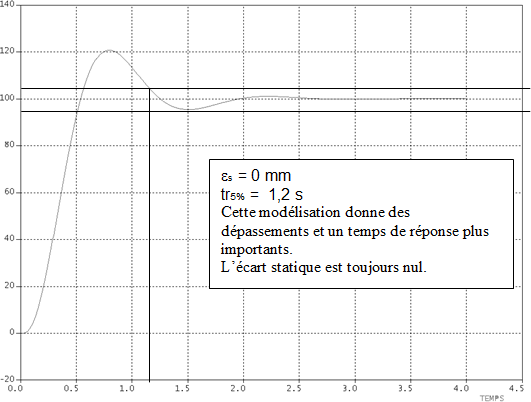
\includegraphics[width=.75\textwidth]{png/q14}
\end{center}
\end{corrige}}{}

\ifthenelse{\boolean{prof}}{}{
\subsection{Annexe}

\begin{center}
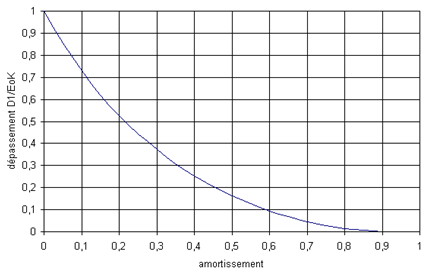
\includegraphics[width=.75\textwidth]{png/fig7}
\end{center}

\begin{center}
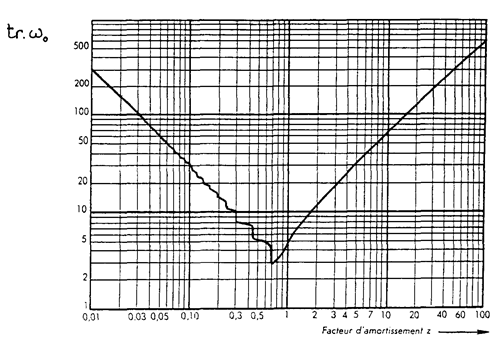
\includegraphics[width=.75\textwidth]{png/fig8}
\end{center}

\subsection{Document réponse}

\begin{center}
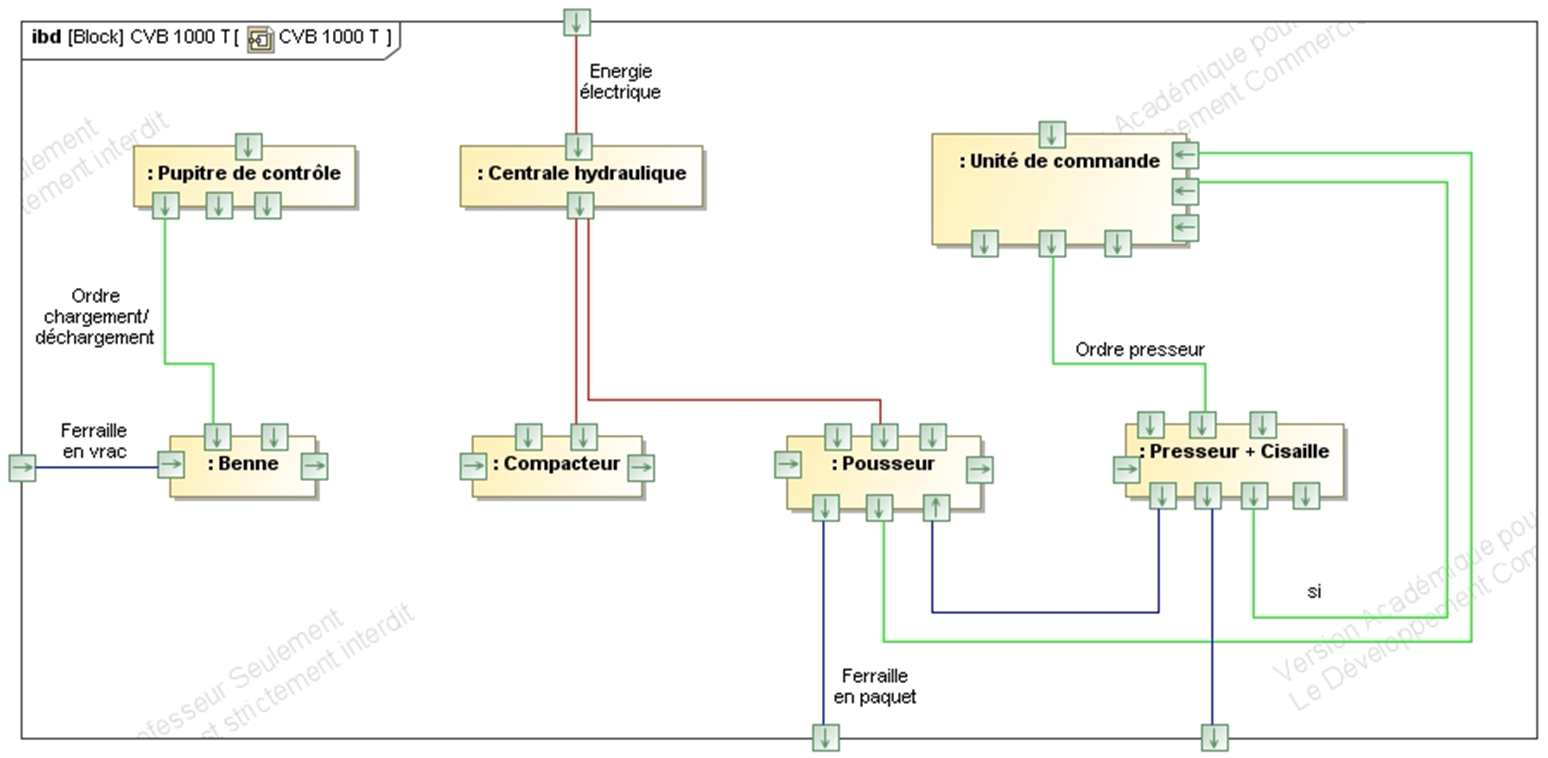
\includegraphics[width=\textwidth]{png/fig9}
\end{center}

\begin{center}
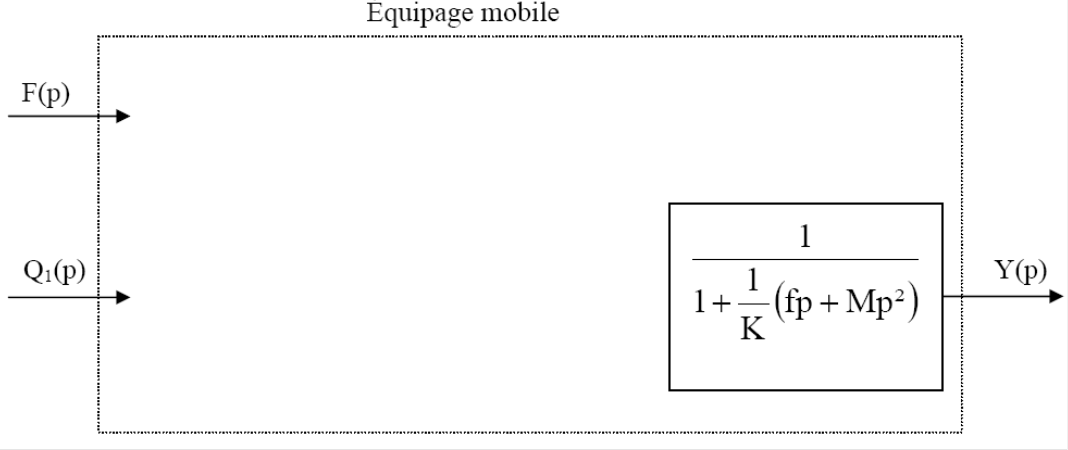
\includegraphics[width=.75\textwidth]{png/fig10}
\end{center}


\begin{center}
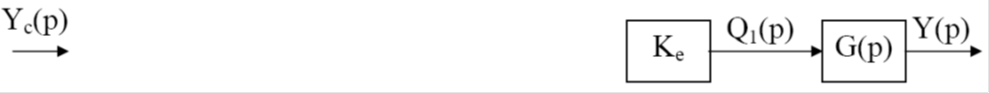
\includegraphics[width=.75\textwidth]{png/fig11}
\end{center}

\begin{center}
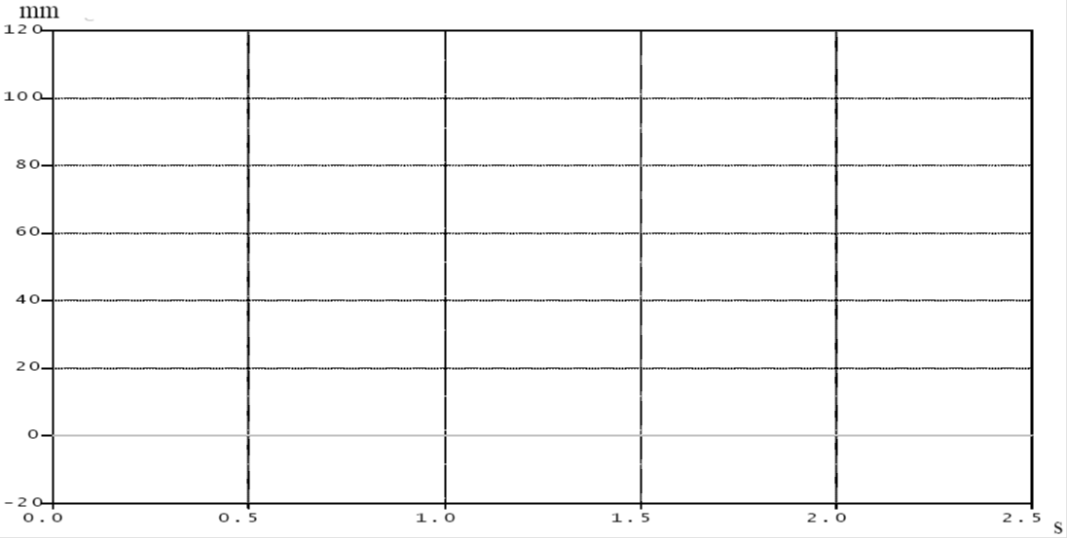
\includegraphics[width=.75\textwidth]{png/fig12}
\end{center}

\begin{center}
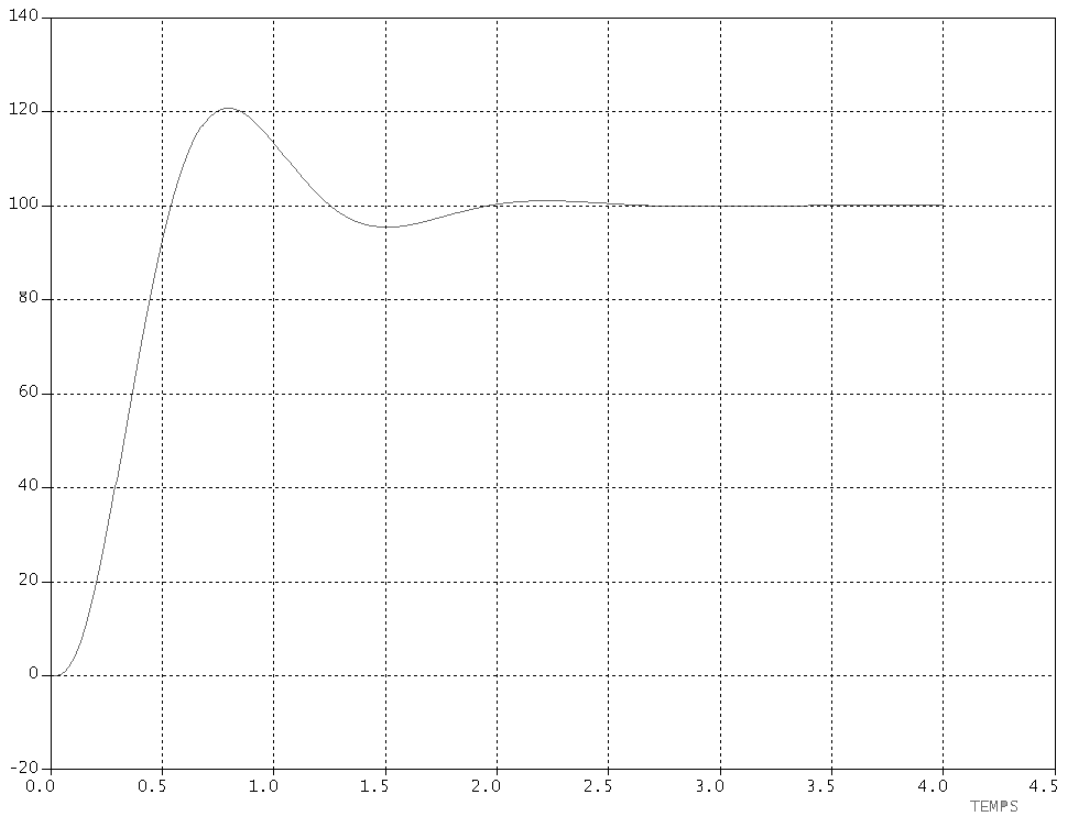
\includegraphics[width=.75\textwidth]{png/fig13}
\end{center}
}



\section{Carrousel au triple mouvement}
\setcounter{subparagraph}{0}
%\textbf{Objectif technologique:} 
%\begin{itemize}
%\item Calculer le rapport de réduction d'un train d'engrenages
%\end{itemize}
\ifthenelse{\boolean{prof}}{}{
\begin{center}
 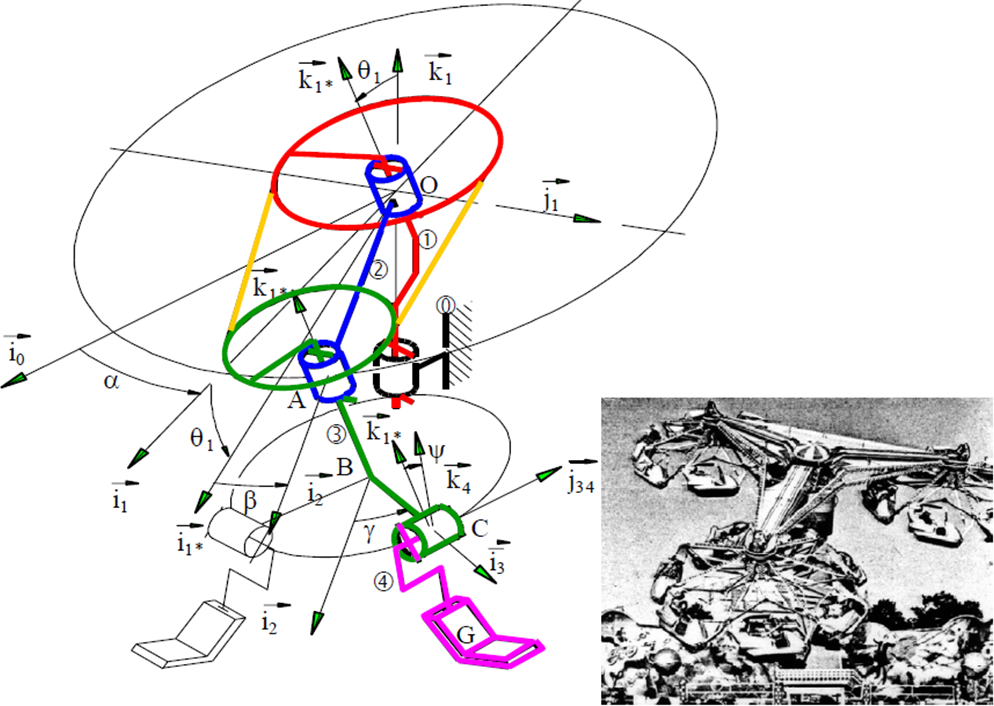
\includegraphics[width=\textwidth]{png/exo1}
\end{center}

Le carrousel étudié est constitué d'un fût 1 supportant un plateau tournant 2 sur lequel sont articulés des disques 3 auxquels sont liées les nacelles 4. 
\subsubsection*{Données}
\begin{itemize}
\item $\mathcal{R}_0 (O,\vect{i_0},\vect{j_0},\vect{k_{01}})$ repère lié au bâti $0$
\item $\mathcal{R}_1 (O,\vect{i_1},\vect{j_1},\vect{k_1})$ et $\mathcal{R}_1^* (O,\vect{i_1^*},\vect{j_1^*},\vect{k_1^*})$ repères liés à $1$
\item $\mathcal{R}_2 (O,\vect{i_2},\vect{j_2},\vect{k_2})$ repère lié à $2$
\item $\mathcal{R}_3 (C,\vect{i_3},\vect{j_3},\vect{k_3})$ repère lié à $3$
\item $\mathcal{R}_4 (C,\vect{i_4},\vect{j_4},\vect{k_4})$ repère lié à $4$
\end{itemize}

$$
\vect{OA}=L\vect{i_2} \quad \vect{AB}=h\vect{k_1^*} \quad \vect{BC}=R\vect{i_3} \quad \vect{GC}=e\vect{k_4} 
$$

$L$, $h$, $R$ et $e$ sont des constantes positives.

\begin{itemize}
\item Liaison 1--0 : pivot d'axe $(O,\vect{k_{01}})$ : $\alpha = (\vect{i_0},\vect{i_1})$
\item Liaison 1--2 : pivot d'axe $(O,\vect{k_{21}^*})$ : $\beta = (\vect{i_1^*},\vect{i_2})$
\item Liaison 3--2 : pivot d'axe $(A,\vect{k_{321}^*})$ : $\gamma = (\vect{i_2},\vect{i_3})$
\item Liaison 4--3 : pivot d'axe $(C,\vect{j_{43}})$ : $\psi = (\vect{k_{321}^*},\vect{k_4})$
\end{itemize}

Inclinaison du plateau 1 : rotation d'axe $(O,\vect{j_1})$, $\theta_1=(\vect{i_1},\vect{i_1^*})$ où $\theta_1$ est une constante positive. La liaison 1--0 n'est pas animée; donc $\alpha=\dot{\alpha}=0$. Un moteur permet d'animer la liaison 2--1 ($\beta\neq0$). 


\begin{center}
 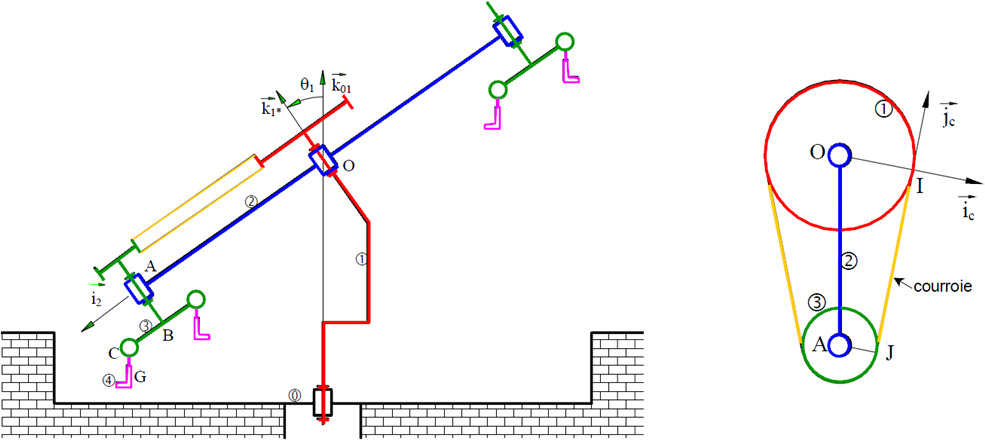
\includegraphics[width=\textwidth]{png/exo2}
\end{center}
}

\subparagraph{}
%\textit{Exprimer $\torseurcin{V}{2}{1}$ au point $A$.}
\textit{Exprimer $\vecto{2}{1}$ et $\vectv{A}{2}{1}$.}
\ifthenelse{\boolean{prof}}{
\begin{corrige}
Les solides $S_2$ et $S_1$ sont en liaison pivot de centre $O$, d'angle $\beta$ et d'axe $\vect{k_{21}}$. En conséquence en $O$, on a :
$$
\left\{
\mathcal{V}(2/1)
\right\}
=
\left\{
\begin{array}{c}
\vect{\Omega(2/1)} = \dot{\beta} \vect{k_{21}} \\
\vect{V(O,2/1)} = \vect{0}
\end{array}
\right\}_O
=
\left\{
\begin{array}{c}
\vect{\Omega(2/1)} = \dot{\beta} \vect{k_{21}} \\
\vect{V(A,2/1)} = \vect{V(O,2/1)} + \vect{AO} \wedge \vect{\Omega(2/1)}
\end{array}
\right\}_A
$$

$$
\vect{V(A,2/1)} = -L\vect{i_2} \wedge  \dot{\beta} \vect{k_{21^*}} = L\dot{\beta}\vect{j_2}
$$

\end{corrige}}{}


\subparagraph{}
%\textit{Exprimer $\torseurcin{V}{3}{1}$ au point $C$.}
\textit{Exprimer $\vecto{3}{1}$ et $\vectv{C}{3}{1}$.}
\ifthenelse{\boolean{prof}}{
\begin{corrige}

Pour calculer la vitesse relative entre $S_3$ et $S_1$, il faut décomposer le torseur cinématique : 
$\left\{
\mathcal{V}(3/1)
\right\} =
\left\{
\mathcal{V}(3/2)
\right\} +
\left\{
\mathcal{V}(2/1)
\right\} 
$

Les solides $S_3$ et $S_2$ sont en liaison pivot de centre $A$, d'angle $\gamma$ et d'axe $\vect{k_{321^*}}$; donc : 
$$
\left\{
\mathcal{V}(3/2)
\right\}
=
\left\{
\begin{array}{c}
\vect{\Omega(3/2)} = \dot{\gamma} \vect{k_{321^*}} \\
\vect{V(A,3/2)} = \vect{0}
\end{array}
\right\}_A
$$

On a donc :
$$
\left\{
\mathcal{V}(3/1)
\right\}
=
\left\{
\begin{array}{c}
\vect{\Omega(3/1)} = \left( \dot{\beta} +\dot{\gamma} \right)\vect{k_{321^*}} \\
\vect{V(A,3/1)} = L\dot{\beta}\vect{j_2}
\end{array}
\right\}_A
$$

En conséquences, 

$$
\vect{V(C,3/1)} = \vect{V(A,3/1)} + \vect{CA} \wedge \vect{\Omega(3/1)} =L\dot{\beta}\vect{j_2} + \left( -R\vect{i_{3}} - h \vect{k_{1^*}}\right) \wedge \left( \dot{\beta} +\dot{\gamma} \right)\vect{k_{321^*}}
$$

$$
\vect{V(C,3/1)} = L\dot{\beta}\vect{j_2} + R \left( \dot{\beta} +\dot{\gamma} \right)\vect{j_3} 
$$
\end{corrige}}{}


\subparagraph{}
%\textit{Exprimer $\torseurcin{V}{4}{1}$ au point $G$.}
\textit{Exprimer $\vectv{G}{4}{1}$.}
\ifthenelse{\boolean{prof}}{
\begin{corrige}En prenant un peu de recul, il n'est pas forcément indispensable d'écrire entièrement le torseur cinématique. Par exemple, dans le cas de $\vect{V(G,4/1)}$ :
$$
\vect{V(G,4/1)} = \vect{V(C,4/1)} + \vect{GC} \wedge \vect{\Omega(4/1)} =
\underbrace{\vect{V(C,4/3)}}_{\vect{0}} + \vect{V(C,3/1)} + \vect{GC} \wedge \underbrace{\vect{\Omega(4/1)}}_{\vect{\Omega(4/3)}+\vect{\Omega(3/1)}}
$$

$$
\vect{V(G,4/1)} =
 L\dot{\beta}\vect{j_2} + R \left( \dot{\beta} +\dot{\gamma} \right)\vect{j_3} 
+ e \vect{k_4} \wedge \left( 
\left( \dot{\beta} +\dot{\gamma} \right)\vect{k_{321^*}}
+\dot{\psi} \vect{j_{43}}
\right)
$$

On a : 
$$ 
\vect{k_4} \wedge \vect{k_{321^*}} = - \sin \psi \vect{j_{43}}  
 $$

$$
\vect{k_4} \wedge \vect{j_{43}} = -\vect{i_{4}}
$$

On a donc :
$$
\vect{V(G,4/1)} =
 L\dot{\beta}\vect{j_2} + R \left( \dot{\beta} +\dot{\gamma} \right)\vect{j_3} 
- e \left( \dot{\beta} +\dot{\gamma} \right)\sin \psi \vect{j_{43}}  
- e \dot{\psi} \vect{i_{4}}
$$

$$
\vect{V(G,4/1)} =
 L\dot{\beta}\vect{j_2} + \left( R -e \sin \psi \right) \left( \dot{\beta} +\dot{\gamma} \right)\vect{j_3} 
- e \dot{\psi} \vect{i_{4}}
$$
\end{corrige}}{}

%\subparagraph{}
%\textit{Exprimer $\vect{V(A,2/1)}$ en fonction de $\dot{\beta}$ et $L$, $\vect{V(C,3/1)}$ en fonction de $R$, $L$, $\dot{\beta}$ et $\dot{\gamma}$ et $\vect{V(G,4/1)}$ en fonction de $R$, $L$, $e$, $\psi$, $\dot{\psi}$, $\dot{\beta}$et $\dot{\gamma}$.}

\vspace{.5cm}

Le fût 1 est muni d'une poulie de diamètre $D$ sur laquelle s'enroule une courroie qui entraîne en rotation la poulie de diamètre $D/2$ liée au disque 3 lors du mouvement de 2 par rapport à 1. 

On a les hypothèses suivantes : 
\begin{itemize}
\item non glissement entre la courroie et les poulies;
\item la courroie est inextensible.
\end{itemize}

De plus le siège 4 est bloqué dans la position $\psi = -\pi/2$ par rapport au disque 3. 

\subparagraph{}
\textit{En utilisant les hypothèses précédentes, montrer que  $\dot{\gamma}=-2\dot{\beta}$.}

\ifthenelse{\boolean{prof}}{
\begin{corrige}
En considérant l'hypothèse de roulement sans glissement au point $I$, le point $I$ est immobile  lorsqu'on considère le mouvement de la courroie (notée c) par rapport à la poule 1 :
$$
\vect{V(I,c/1)} = \vect{0}
$$

En utilisant la décomposition du vecteur vitesse : 
$$
\vect{V(I,c/1)} = \vect{V(I,c/2)} + \vect{V(I,2/1)}
$$

En conséquence, 
$$
\vect{V(I,c/2)}= -\vect{V(I,2/1)}
$$

Par ailleurs, 
$$
\vect{V(I,2/1)} = \vect{V(O,2/1)} + \vect{IO} \wedge \vect{\Omega(2/1)} = 
0 -\dfrac{D}{2}\vect{i_c} \wedge \dot{\beta} \vect{k_{321^*}} = \dfrac{D}{2}\dot{\beta}\vect{j_c}
$$

De même, en considérant l'hypothèse de roulement sans glissement au point $J$, le point $J$ est immobile  lorsqu'on considère le mouvement de la courroie (notée c) par rapport à la poule 3 :
$$
\vect{V(J,c/3)} = \vect{0}
$$


En utilisant la décomposition du vecteur vitesse : 
$$
\vect{V(J,c/3)} = \vect{V(J,c/2)} + \vect{V(J,2/3)}
$$

En conséquence, 
$$
\vect{V(J,c/2)}= -\vect{V(J,2/3)}
$$
Par ailleurs, 
$$
\vect{V(J,2/3)} = \vect{V(A,2/3)} + \vect{JO} \wedge \vect{\Omega(2/3)} = 
0 -\dfrac{D}{4}\vect{i_c} \wedge -\dot{\gamma} \vect{k_{321^*}} = - \dfrac{D}{4}\dot{\gamma}\vect{j_c}
$$


La courroie étant inextensible, 
$$ \vect{V(I,c/2)}= \vect{V(J,c/2)}$$
Et donc : 
$$
\dot{\gamma} = -2 \dot{\beta}
$$

\end{corrige}}{}

\subparagraph{}
\textit{En déduire la nouvelle expression de $\vect{V(G,4/1)}$ en fonction de $R$, $L$, $e$ et $\dot{\beta}$.}
\ifthenelse{\boolean{prof}}{
\begin{corrige}

On a donc $\dot{\psi}=0$ et :

$$
\vect{V(G,4/1)} =
 L\dot{\beta}\vect{j_2} -\dot{\beta} \left( R +e\right) \vect{j_3} 
$$



\end{corrige}}{}

\subparagraph{}
\textit{Exprimer l'accélération du point $G$ dans le mouvement de 4/1 en fonction de $R$, $L$, $e$, $\dot{\beta}$ si $\dot{\beta}$ est constant.}
\ifthenelse{\boolean{prof}}{
\begin{corrige}

$$
\vect{\Gamma(G,4/1)}  =\left[\dfrac{d\vect{V(G,4/1)}}{dt}\right]_{\mathcal{R}_1}
=
L\underbrace{\ddot{\beta}}_{0}\vect{j_2} 
+ L\dot{\beta}\left[\dfrac{d\vect{j_2}}{dt}\right]_{\mathcal{R}_1}
-\underbrace{\ddot{\beta}}_{0} \left( R +e\right) \vect{j_3} 
 -\dot{\beta} \left( R +e\right) \left[\dfrac{d\vect{j_3}}{dt}\right]_{\mathcal{R}_1}
$$

$$
\left[\dfrac{d\vect{j_2}}{dt}\right]_{\mathcal{R}_1}  =
\left[\dfrac{d\vect{j_2}}{dt}\right]_{\mathcal{R}_2} + \vect{\Omega(2/1)}\wedge \vect{j_2}
=\vect{0} + \dot{\beta}\vect{k_{21^*}} \wedge \vect{j_2}
=- \dot{\beta}\vect{i_2}
$$


$$
\left[\dfrac{d\vect{j_3}}{dt}\right]_{\mathcal{R}_1}  =
\left[\dfrac{d\vect{j_3}}{dt}\right]_{\mathcal{R}_3} + \vect{\Omega(3/1)}\wedge \vect{j_3}
=\vect{0} + (\dot{\beta}+\dot{\gamma})\vect{k_{321^*}} \wedge \vect{j_3}
=\dot{\beta} \vect{i_3}
$$

$$
\vect{\Gamma(G,4/1)} 
=
- L\dot{\beta}^2 \vect{i_2}
 -\dot{\beta}^2  \left( R +e\right) \vect{i_3}
$$

\end{corrige}}{}

\subparagraph{}
\textit{Calculer la valeur maximale de la norme de cette accélération pour $\dot{\beta}=2 rad/s$, $L=5m$, $R=1m$, $e=1m$.}
\ifthenelse{\boolean{prof}}{
\begin{corrige}

On a :
$$
||\vect{\Gamma(G,4/1)}||^2
= L^2\dot{\beta}^4 +\dot{\beta}^4  \left( R +e\right)^2
+2 L\dot{\beta}^4 \left( R +e\right) \cos (\vect{i_2},\vect{i_3})
= L^2\dot{\beta}^4 +\dot{\beta}^4  \left( R +e\right)^2
+2 L\dot{\beta}^4 \left( R +e\right) \cos \gamma
$$

$||\vect{\Gamma(G,4/1)}||^2$ est maximal lorsque $\cos \gamma = 1$; donc
$$||\vect{\Gamma(G,4/1)}|| = \sqrt{L^2\dot{\beta}^4 +\dot{\beta}^4  \left( R +e\right)^2
+2 L\dot{\beta}^4 \left( R +e\right) }
= \dot{\beta}^2(L+R+e) = 28\;m\cdot s^{-2}
$$

\end{corrige}}{}

Le dessin ci-dessous montre le mécanisme permettant de faire varier en fonctionnement l'angle $\theta_1$. L'actionneur de ce mécanisme est le vérin hydraulique 5--6. 

Soit $\vect{FH}=2a\vect{i_7}$, $\vect{FE}=3a\vect{i_1}$ (où $a$ est une constante positive); $\vect{EH}=x(t)\vect{i_{56}}$ et $\varphi(t)=(\vect{i_7},\vect{i_1})$.

\subparagraph{}
\textit{Exprimer $x$ en fonction de $a$ et $\varphi$ puis la vitesse de sortie de la tige du vérin, soit $\vect{V(H,6/5)}$, en fonction de $a$, $\varphi$ et $\dot{\varphi}$.}
\ifthenelse{\boolean{prof}}{
\begin{corrige}

Commençons par écrire la fermeture de chaîne cinématique dans le triangle EFH : 
$$ 
\vect{EF}+\vect{FH}+\vect{HE}=\vect{0}
\Longleftrightarrow
x(t)\vect{i_{56}}=2a\vect{i_7}-3a\vect{i_1}
$$
En élevant cette relation au carré, on a : 
$$
x(t)^2 = 4a^2 + 9a^2 - 12a^2\cos\phi
$$

En conséquence, 
$$
x(t)=a\sqrt{13- 12\cos\phi}
$$

Par ailleurs, 
$$
\vect{V(H,6/5)} = \left[\dfrac{d\vect{EH}}{dt}\right]_{\mathcal{R}_5} = 
\dfrac{d(a\sqrt{13- 12\cos\phi})}{dt} \vect{i_{56}}
$$

$$
\vect{V(H,6/5)} = 
\dfrac{6a\dot{\phi}\sin\phi}{\sqrt{13-12\cos\phi}}
\vect{i_{56}}
$$

\end{corrige}}{}


\subparagraph{}
\textit{En considérant que dans cet intervalle de temps, $\dot{\varphi}$ est constante, déterminer le volume d'huile nécessaire au passage de la position $\varphi=\pi/9$ à la position $\varphi=\pi/3$, si $S$ est la section du piston sur laquelle agit l'huile.}
\ifthenelse{\boolean{prof}}{
\begin{corrige}
$$
Vol = S\cdot\left(x\left(\dfrac{\pi}{9}\right) - x\left(\dfrac{\pi}{6}\right)\right) = 0,187\;m^3
$$

\end{corrige}}{}


AN : $a=2m$, $S=700cm^2$.

\begin{center}
 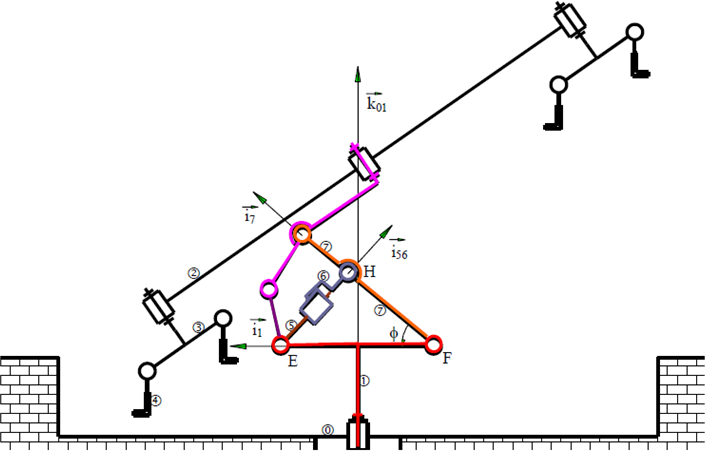
\includegraphics[width=\textwidth]{png/exo3}
\end{center}



\end{document}



\subparagraph{}
\textit{}
\ifthenelse{\boolean{prof}}{
\begin{corrige}
\end{corrige}}{}


